\documentclass[a4paper]{article}

\usepackage{verbatim}
\usepackage{tikz}
\usepackage{mathpazo}
\usepackage{bm}
\usetikzlibrary{calc, external, intersections, through}
%\tikzexternalize[prefix=tikz/]

\textwidth=15.5cm
\textheight=23cm
\topmargin=0pt
\headheight=0pt
\oddsidemargin=1em
\headsep=0pt
\parindent=0pt

\begin{document}
\thispagestyle{empty}

\begin{center}
\textbf{\sffamily \Large Visualization of Theorems of Geometry}

\bigskip

\textbf{\sffamily \large Moti Ben-Ari}

\bigskip

\textbf{\sffamily \large http://www.weizmann.ac.il/sci-tea/benari/}

\end{center}

\textsf{\footnotesize \copyright{} 2017-8 by Moti Ben-Ari. This work is licensed under the Creative Commons Attribution-ShareAlike 3.0 Unported License. To view a copy of this license, visit http://creativecommons.org/licenses/by-sa/3.0/ or send a letter to Creative Commons, 444 Castro Street, Suite 900, Mountain View, California, 94041, USA.}

\bigskip

%%%%%%%%%%%%%%%%%%%%%%%%%%%%%%%%%%%%%%%%%%%%%%%%%%%%%%%%%

This document contains a list of advanced theorems of plane geometry that are presented visually.

\begin{center}
\Large\sffamily\bfseries Triangles
\end{center}

% Thale's theorem 1
%
\begin{minipage}[t]{.45\textwidth}
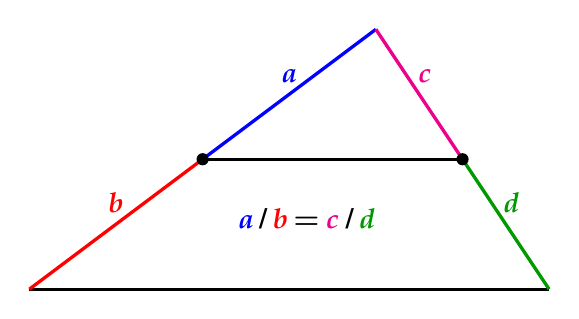
\begin{tikzpicture}[scale=1.1]
% Points of the triangle
\coordinate (a) at (0,0);
\coordinate (b) at (6,0);
\coordinate (c) at (4,3);
% Midpoints of the sides
\coordinate (mid1) at ($(a)!.5!(c)$);
\coordinate (mid2) at ($(b)!.5!(c)$);
% Draw the base and median
\draw[very thick] (a) -- (b);
\draw[very thick] (mid1) -- (mid2);
% Get the median
\coordinate (midbase) at ($(a)!.5!(b)$);
% Draw the triangle, sides in two parts
\draw[very thick,red] (a) -- node[above] {$\bm{b}$} (mid1);
\draw[very thick,blue] (mid1) -- node[above] {$\bm{a}$} (c);
\draw[very thick,green!60!black] (b) -- node[above,xshift=2pt] {$\bm{d}$} (mid2);
\draw[very thick,magenta] (mid2) -- node[above,xshift=2pt] {$\bm{c}$} (c);
% Dots at the midpoints
\fill (mid1) circle (2pt);
\fill (mid2) circle (2pt);
% Display formula in color
\begin{scope}[xshift=2.5cm,yshift=.7cm]
\node[anchor=base,blue] at (0,0) {$\bm{a}$};
\node[anchor=base] at (.2,0) {$\bm{/}$};
\node[anchor=base,red] at (.4,0) {$\bm{b}$};
\node[anchor=base] at (.7,0) {$\bm{=}$};
\node[anchor=base,magenta] at (1,0) {$\bm{c}$};
\node[anchor=base] at (1.2,0) {$\bm{/}$};
\node[anchor=base,green!60!black] at (1.4,0) {$\bm{d}$};
\end{scope}
\end{tikzpicture}

\smallskip\sffamily
\centering Thales theorem.
\end{minipage}
\hspace{.1\textwidth}
% Thale's theorem 2
%
\begin{minipage}[t]{.45\textwidth}
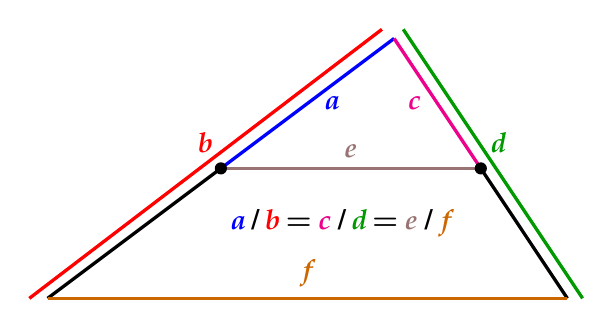
\begin{tikzpicture}[scale=1.1]
% Points of the triangle
\coordinate (a) at (0,0);
\coordinate (b) at (6,0);
\coordinate (c) at (4,3);
% Midpoints of the sides
\coordinate (mid1) at ($(a)!.5!(c)$);
\coordinate (mid2) at ($(b)!.5!(c)$);
% Midpoint of the base
\coordinate (midbase) at ($(a)!.5!(b)$);
\draw[very thick] (a) -- (mid1);
\draw[very thick,blue] (mid1) -- node[right,xshift=2pt] {$\bm{a}$} (c);
\draw[very thick] (b) -- (mid2);
\draw[very thick,magenta] (mid2) -- node[left,xshift=-2pt] {$\bm{c}$} (c);
% Draw the offest lines
\draw[very thick,red]
  let \p1 = (a), \p2 = (c) in
    (\x1-6pt,\y1) -- node[above] {$\bm{b}$} (\x2-4pt,\y2+3pt);
\draw[very thick,green!60!black]
  let \p1 = (b), \p2 = (c) in
    (\x1+5pt,\y1) -- node[above,xshift=2pt] {$\bm{d}$} (\x2+3pt,\y2+3pt);
% Draw the base and median
\draw[very thick,orange!80!black] (a) -- node[above] {$\bm{f}$} (b);
\draw[very thick,pink!60!black] (mid1) -- node[above] {$\bm{e}$} (mid2);
% Points at the midpoints
\fill (mid1) circle (2pt);
\fill (mid2) circle (2pt);
% Display formula in color
\begin{scope}[xshift=2.2cm,yshift=.8cm]
\node[anchor=base,blue] at (0,0) {$\bm{a}$};
\node[anchor=base] at (.2,0) {$\bm{/}$};
\node[anchor=base,red] at (.4,0) {$\bm{b}$};
\node[anchor=base] at (.7,0) {$\bm{=}$};
\node[anchor=base,magenta] at (1,0) {$\bm{c}$};
\node[anchor=base] at (1.2,0) {$\bm{/}$};
\node[anchor=base,green!60!black] at (1.4,0) {$\bm{d}$};
\node[anchor=base] at (1.7,0) {$\bm{=}$};
\node[anchor=base,pink!60!black] at (2,0) {$\bm{e}$};
\node[anchor=base] at (2.2,0) {$\bm{/}$};
\node[anchor=base,orange!80!black] at (2.4,0) {$\bm{f}$};
\end{scope}
\end{tikzpicture}

\smallskip\sffamily
\centering Thales theorem.
\end{minipage}

\bigskip
\bigskip

%
% Angle bisector splits opposite side at same ratio as sides
%
\begin{minipage}[t]{.45\textwidth}
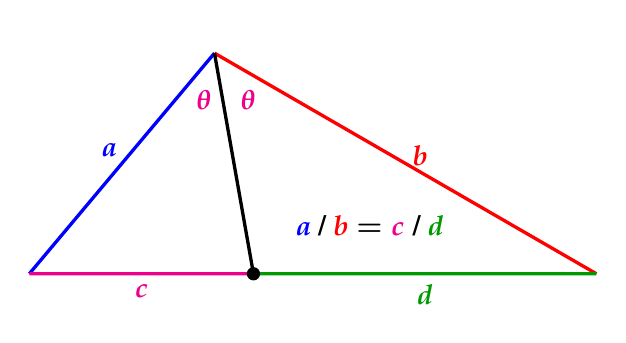
\begin{tikzpicture}[baseline=-4mm,scale=1.2]
% Draw base and path two lines at known angles
\path[name path=ab] (0,0) coordinate (a) -- (0:6) coordinate (b);
\path[name path=ac] (a) -- node[left,xshift=-2pt,blue] {$\bm{a}$} +(50:3.4);
\path[name path=bc] (b) -- node[right,xshift=4pt,red] {$\bm{b}$} +(150:5);
% Get their intersection and draw lines to third vertex
\path[name intersections={of=ac and bc,by=c}];
\draw[blue,very thick] (a) -- (c);
\draw[red,very thick] (c) -- (b);
% Path bisectors of two lines
\path[name path=bisector] (c) -- +(-80:2.5);
% Intersection of angle bisectors
\path [name intersections={of=bisector and ab,by=int}];
% Draw base of triangle
\draw[very thick,magenta] (a) -- node[below] {$\bm{c}$} (int);
\draw[very thick,green!60!black] (int) -- node[below] {$\bm{d}$} (b);
% Draw bisector and label angle
\draw[very thick] (c) -- (int);
\node[magenta,below,xshift=-4pt,yshift=-10pt] at (c) {$\bm{\theta}$};
\node[magenta,below,xshift=12pt,yshift=-10pt] at (c) {$\bm{\theta}$};
 Draw dot
\fill (int) circle (2pt);
% Display formula in color
\begin{scope}[xshift=29mm,yshift=4mm]
\node[anchor=base,blue] at (0,0) {$\bm{a}$};
\node[anchor=base] at (.2,0) {$\bm{/}$};
\node[anchor=base,red] at (.4,0) {$\bm{b}$};
\node[anchor=base] at (.7,0) {$\bm{=}$};
\node[anchor=base,magenta] at (1,0) {$\bm{c}$};
\node[anchor=base] at (1.2,0) {$\bm{/}$};
\node[anchor=base,green!60!black] at (1.4,0) {$\bm{d}$};
\end{scope}
\end{tikzpicture}

\smallskip\sffamily
\centering
Angle bisector splits the opposite side.
\end{minipage}
\hspace{.1\textwidth}
% Median of a triangle is half the base
%
\begin{minipage}[t]{.45\textwidth}
\hspace{1em}
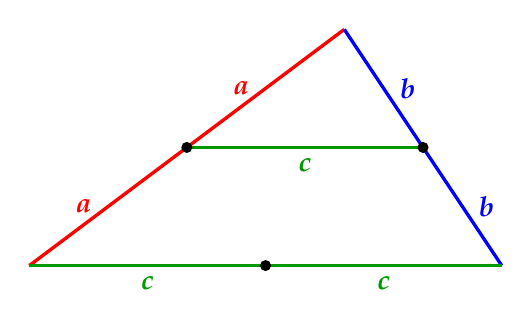
\begin{tikzpicture}
% Points of the triangle
\coordinate (a) at (0,0);
\coordinate (b) at (6,0);
\coordinate (c) at (4,3);
% Midpoints of the sides
\coordinate (mid1) at ($(a)!.5!(c)$);
\coordinate (mid2) at ($(b)!.5!(c)$);
% Midpoint of the base
\coordinate (midbase) at ($(a)!.5!(b)$);
% Draw the sides of the triangle: the base is drawn in two parts
\draw[very thick,red] (a) -- node[left,xshift=-2pt] {$\bm{a}$} (mid1);
\draw[very thick,red] (mid1) -- node[left,xshift=-2pt] {$\bm{a}$} (c);
\draw[very thick,blue] (b) -- node[right,xshift=2pt] {$\bm{b}$} (mid2);
\draw[very thick,blue] (mid2) -- node[right,xshift=2pt] {$\bm{b}$} (c);
% Draw the median
\draw[very thick,green!60!black] (mid1) -- node[below] {$\bm{c}$} (mid2);
% Draw the base
\draw[very thick,green!60!black] (a) -- node[below] {$\bm{c}$} (midbase);
\draw[very thick,green!60!black] (b) -- node[below] {$\bm{c}$} (midbase);
% Draw dots at the midpoints
\fill (mid1) circle (2pt);
\fill (mid2) circle (2pt);
\fill (midbase) circle (2pt);
\end{tikzpicture}

\smallskip\sffamily
\centering
Bisector of sides adjacent to an angle.
\end{minipage}

\bigskip
\bigskip

% Bisector of the hypotenuse is half the hypotenuse
%
\begin{minipage}[t]{.45\textwidth}
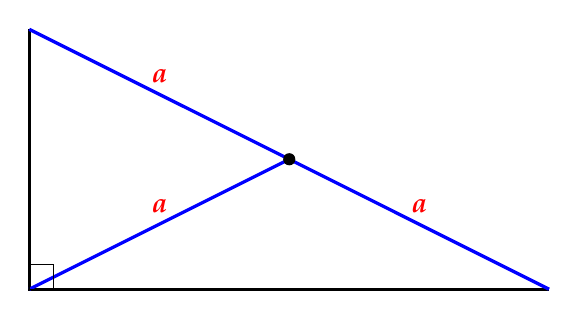
\begin{tikzpicture}[scale=1.1]
\coordinate (a) at (0,0);   % Points of the triangle
\coordinate (b) at (6,0);
\coordinate (c) at (0,3);
% Coordinate of bisector
\coordinate (hyp) at ($(b)!.5!(c)$);
% Draw the triangle and bisectors
\draw[very thick] (b) -- (a) -- (c);
\draw[very thick,blue] (a) -- node[above,red] {$\bm{a}$} (hyp);
\draw[very thick,blue] (b) -- node[above,red] {$\bm{a}$} (hyp);
\draw[very thick,blue] (c) -- node[above,red] {$\bm{a}$} (hyp);
% Draw square to denote right angle
\draw (a) rectangle +(8pt,8pt);
% Points at the intersections
\fill (hyp) circle (2pt);
\end{tikzpicture}

\smallskip\sffamily
\centering
Bisector of the hypotenuse.
\end{minipage}
\hspace{.1\textwidth}
% Medians of a triangle meet at a point with ratio 1:2
%
\begin{minipage}[t]{.45\textwidth}
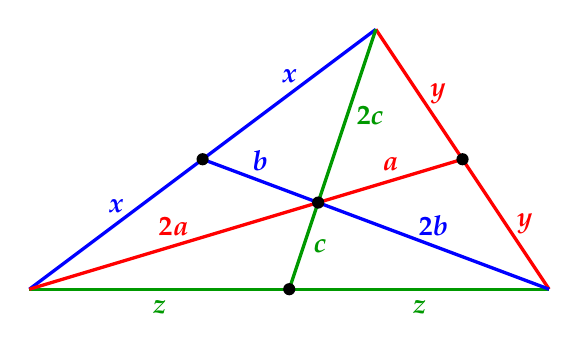
\begin{tikzpicture}[scale=1.1]
\coordinate (a) at (0,0);   % Points of the triangle
\coordinate (b) at (6,0);
\coordinate (c) at (4,3);
% Coordinates of bisectors
\coordinate (ab) at ($(a)!.5!(b)$);
\coordinate (bc) at ($(b)!.5!(c)$);
\coordinate (ac) at ($(a)!.5!(c)$);
% Draw the triangle and bisectors
\draw[blue,very thick] (a) -- node[above] {$\bm{x}$} (ac) -- node[above] {$\bm{x}$} (c);
\draw[red,very thick] (b) -- node[right] {$\bm{y}$} (bc) -- node[right] {$\bm{y}$} (c);
\draw[green!60!black,very thick] (a) -- node[below] {$\bm{z}$} (ab) -- node[below] {$\bm{z}$} (b);
\draw[very thick,red,name path=da] (a) -- (bc);
\draw[very thick,blue,name path=db] (b) -- (ac);
\draw[very thick,green!60!black,name path=dc] (c) -- (ab);
% Get their intersection
\path [name intersections={of=da and db,by={intersection}}];
% Labels
\path (a) -- node[above,red] {$\bm{2a}$} (intersection);
\path (bc) -- node[above,red] {$\bm{a}$} (intersection);
\path (b) -- node[above,blue] {$\bm{2b}$} (intersection);
\path (ac) -- node[above,blue] {$\bm{b}$} (intersection);
\path (c) -- node[right,green!60!black] {$\bm{2c}$} (intersection);
\path (ab) -- node[right,green!60!black] {$\bm{c}$} (intersection);
% Points at the intersections
\fill (intersection) circle (2pt);
\fill (ab) circle (2pt);
\fill (ac) circle (2pt);
\fill (bc) circle (2pt);
\end{tikzpicture}

\smallskip\sffamily
\centering
Intersection of the medians.
\end{minipage}

\bigskip
\bigskip
\bigskip
\bigskip

%
% Area of a triangle
%
\begin{minipage}[t]{.45\textwidth}
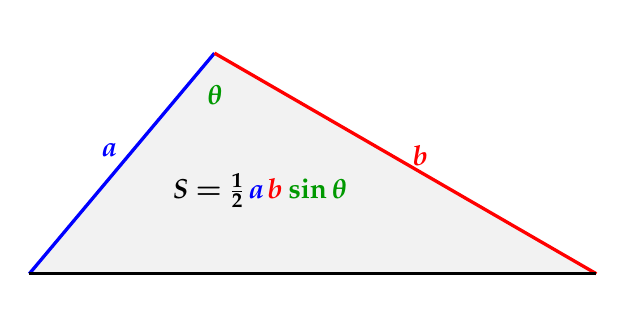
\begin{tikzpicture}[baseline=-4mm,scale=1.2]
% Draw base and path two lines at known angles
\path[name path=ab] (0,0) coordinate (a) -- (0:6) coordinate (b);
\path[name path=ac] (a) -- node[left,xshift=-2pt,blue] {$\bm{a}$} +(50:3.4);
\path[name path=bc] (b) -- node[right,xshift=4pt,red] {$\bm{b}$} +(150:5);
% Get their intersection and draw lines to third vertex
\path[name intersections={of=ac and bc,by=c}];
\path[fill,gray!10] (a) -- (b) -- (c) -- cycle;
\draw[blue,very thick] (a) -- (c);
\draw[red,very thick] (c) -- (b);
\draw[very thick] (a) -- (b);
\node[green!60!black,below,yshift=-8pt] at (c) {$\bm{\theta}$};
% Display formula in color
\begin{scope}[xshift=16mm,yshift=8mm]
\node[anchor=base] at (0,0) {$\bm{S}$};
\node[anchor=base] at (.3,0) {$\bm{=}$};
\node[anchor=base] at (.6,0) {$\bm{\frac{1}{2}}$};
\node[anchor=base,blue] at (.8,0) {$\bm{a}$};
\node[anchor=base,red] at (1,0) {$\bm{b}$};
\node[anchor=base,green!60!black] at (1.45,0) {$\bm{\sin \theta}$};
\end{scope}
\end{tikzpicture}

\smallskip\sffamily
\centering
Area of a triangle.
\end{minipage}
\hspace{.1\textwidth}
\begin{comment}
%
% Law of cosines
%
\begin{minipage}[t]{.45\textwidth}
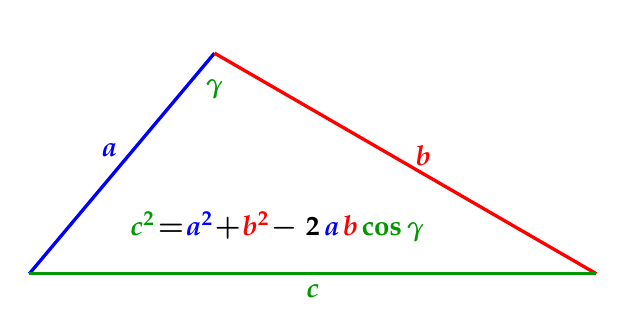
\begin{tikzpicture}[baseline=-4mm,scale=1.2]
% Draw base and path two lines at known angles
\path[name path=ab] (0,0) coordinate (a) -- (0:6) coordinate (b);
\path[name path=ac] (a) -- node[left,xshift=-2pt,blue] {$\bm{a}$} +(50:3.4);
\path[name path=bc] (b) -- node[right,xshift=5pt,red] {$\bm{b}$} +(150:5);
% Get their intersection and draw lines to third vertex
\path[name intersections={of=ac and bc,by=c}];
%\path[fill,gray!20] (a) -- (b) -- (c) -- cycle;
\draw[blue,very thick] (a) -- (c);
\draw[red,very thick] (c) -- (b);
\draw[very thick,green!60!black] (a) -- node[below] {$\bm{c}$} (b);
\node[green!60!black,below,yshift=-6pt] at (c) {$\bm{\gamma}$};
% Display formula in color
\begin{scope}[xshift=12mm,yshift=4mm]
\node[anchor=base,green!60!black] at (0,0) {$\bm{c^2}$};
\node[anchor=base] at (.3,0) {$\bm{=}$};
\node[anchor=base,blue] at (.6,0) {$\bm{a^2}$};
\node[anchor=base] at (.9,0) {$\bm{+}$};
\node[anchor=base,red] at (1.2,0) {$\bm{b^2}$};
\node[anchor=base] at (1.5,0) {$\bm{-}$};
\node[anchor=base] at (1.8,0) {$\bm{2}$};
\node[anchor=base,blue] at (2,0) {$\bm{a}$};
\node[anchor=base,red] at (2.2,0) {$\bm{b}$};
\node[anchor=base,green!60!black] at (2.65,0) {$\bm{\cos \gamma}$};
\end{scope}
\end{tikzpicture}

\smallskip\sffamily
\centering
Law of cosines.
\end{minipage}


\bigskip
\bigskip

%
% Law of sines 1
%
\begin{minipage}[t]{.45\textwidth}
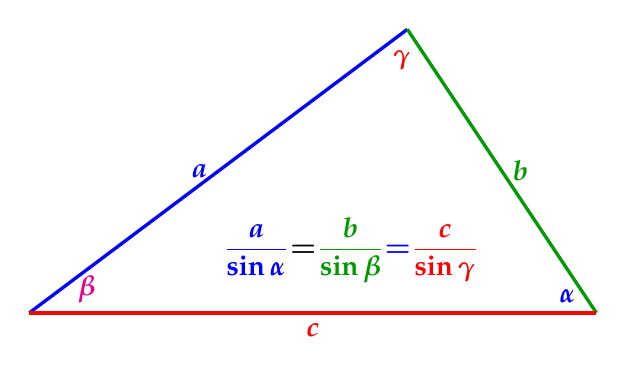
\begin{tikzpicture}[scale=1.2]
\coordinate (a) at (0,0);
\coordinate (b) at (6,0);
\coordinate (c) at (4,3);
% Draw triangle
\draw [very thick,blue] (a) -- node[left] {$\bm{a}$} (c);
\draw[very thick,green!60!black] (c) -- node[right] {$\bm{b}$} (b);
\draw[very thick,red] (a) -- node[below] {$\bm{c}$} (b);
% Label angles
\node[magenta,,above right,xshift=14pt] at (a) {$\bm{\beta}$};
\node[blue,above left,xshift=-4pt] at (b) {$\bm{\alpha}$};
\node[red,below,xshift=-2pt,yshift=-4pt] at (c) {$\bm{\gamma}$};
% Display formula in color
\begin{scope}[xshift=24mm,yshift=6mm]
\node[anchor=base,blue] at (0,0) {$\bm{\displaystyle\frac{a}{\sin \alpha}}$};
\node[anchor=base] at (.5,0) {$\bm{=}$};
\node[anchor=base,green!60!black] at (1,0) {$\bm{\displaystyle\frac{b}{\sin \beta}}$};
\node[anchor=base,blue] at (1.5,0) {$\bm{=}$};
\node[anchor=base,red] at (2,0) {$\bm{\displaystyle\frac{c}{\sin \gamma}}$};
\end{scope}
\end{tikzpicture}

\smallskip\sffamily
\centering
Law of sines.
\end{minipage}
\end{comment}
%\hspace{.1\textwidth}
%
% Law of sines 2
%
\begin{minipage}[t]{.45\textwidth}
%\hspace{3em}
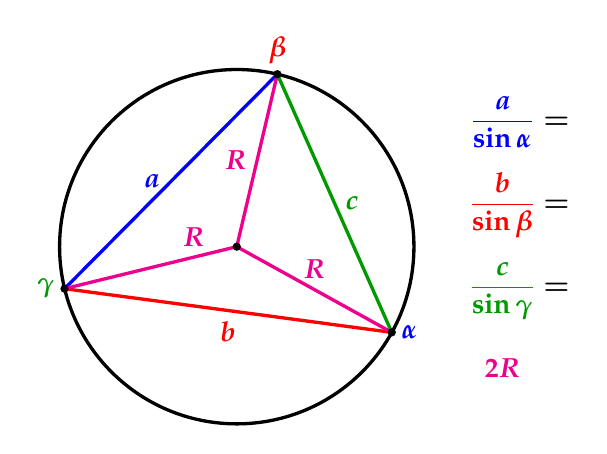
\begin{tikzpicture}[scale=.75]
\coordinate (a) at (0,0);
\coordinate (b) at (6,0);
% Line containing lower points is (c) -- (d)
\coordinate (c) at (0,-.7);
\coordinate (d) at (6,-1.5);
% Line containing upper points is (e) -- (f)
\coordinate (e) at (0,2);
\coordinate (f) at (4,3);
% Name the two chords
\path [name path=chord1] (c) -- (d);
\path [name path=chord2] (e) -- (f);
% Name the coordinate of the center of the circle
\coordinate (center) at ($ (a)!.5!(b) $);
% Draw a circle whose center is half-way between (a) and (b) through (a)
\node [draw,very thick,circle through=(a),name path=circ] at (center) {};
% Get intersections of the upper and lower lines with the circle
\path [name intersections={of=circ and chord1,by={i1,i2}}];
\path [name intersections={of=circ and chord2,by={i3,i4}}];
% Draw triangle
\draw[very thick,blue] (i1) -- node[left] {$\bm{a}$} (i3);
\draw[very thick,green!60!black] (i3) -- node[right] {$\bm{c}$} (i2);
\draw[very thick,red] (i2) -- node[below] {$\bm{b}$} (i1);
% Draw radii
\draw[very thick,magenta] (center) -- node[above,near start] {$\bm{R}$} (i1);
\draw[very thick,magenta] (center) -- node[above] {$\bm{R}$} (i2);
\draw[very thick,magenta] (center) -- node[left] {$\bm{R}$} (i3);
% Label angles
\node[left,green!60!black] at (i1) {$\bm{\gamma}$};
\node[right,blue] at (i2) {$\bm{\alpha}$};
\node[above,red] at (i3) {$\bm{\beta}$};
% Draw dots at all intersections
\fill (i1) circle (2pt);
\fill (i2) circle (2pt);
\fill (i3) circle (2pt);
\fill (center) circle (2pt);
% Display formula in color
\begin{scope}[xshift=75mm,yshift=20mm]
\node[anchor=base,blue] at (0,0) {$\bm{\displaystyle\frac{a}{\sin \alpha}}$};
\node[anchor=base] at (26pt,0) {$\bm{=}$};
\node[anchor=base,red] at (0,-40pt) {$\bm{\displaystyle\frac{b}{\sin \beta}}$};
\node[anchor=base] at (26pt,-40pt) {$\bm{=}$};
\node[anchor=base,green!60!black] at (0,-80pt) {$\bm{\displaystyle\frac{c}{\sin \gamma}}$};
\node[anchor=base] at (26pt,-80pt) {$\bm{=}$};
\node[anchor=base,magenta] at (0,-120pt) {$\bm{2R}$};
\end{scope}
\end{tikzpicture}

\smallskip\sffamily
\centering
Law of sines.
\end{minipage}

\bigskip
\bigskip
\bigskip

% Inscribed circle center at meeting of angle bisectors
%
\begin{minipage}[t]{.45\textwidth}
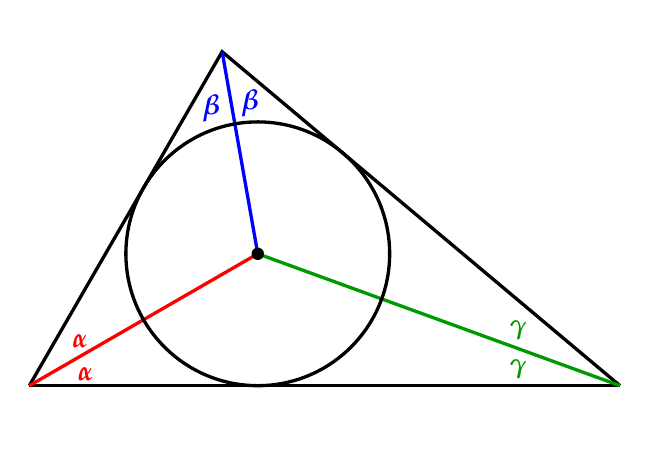
\begin{tikzpicture}[baseline=-6mm,scale=1.5]
% Draw base and path two lines at known angles
\draw[very thick] (0,0) coordinate (a) -- (0:5) coordinate (b);
\path[name path=ac] (a) -- +(60:3.5);
\path[name path=bc] (b) -- +(140:4.5);
% Get their intersection and draw lines to third vertex
\path[name intersections={of=ac and bc,by=c}];
\draw[very thick] (a) -- (c) -- (b);
% Path bisectors of two lines
\path[name path=bia,blue] (a) -- +(30:3.6);
\path[name path=bib,red] (b) -- +(160:5);
% Intersection of angle bisectors
\path [name intersections={of=bia and bib,by=center}];
%% Draw angle bisectors to center
\draw[very thick,red] (a) -- (center);
\draw[very thick,blue] (c) -- (center);
\draw[very thick,green!60!black] (b) -- (center);
%% Labels of angles
\node[red,right,xshift=14pt,yshift=4pt] at (a) {$\bm{\alpha}$};
\node[red,right,xshift=12pt,yshift=16pt] at (a) {$\bm{\alpha}$};
\node[blue,below,xshift=-4pt,yshift=-12pt] at (c) {$\bm{\beta}$};
\node[blue,below,xshift=10pt,yshift=-10pt] at (c) {$\bm{\beta}$};
\node[green!60!black,left,xshift=-30pt,yshift=6pt] at (b) {$\bm{\gamma}$};
\node[green!60!black,left,xshift=-30pt,yshift=20pt] at (b) {$\bm{\gamma}$};
%% Get perpendicular from center to one side and draw circle
\coordinate (perp) at ($(a)!(center)!(b)$);
\node [very thick,draw,circle through=(perp)] at (center) {};
%% Draw dot at center
\fill (center) circle (1.5pt);
\end{tikzpicture}

\smallskip\sffamily
\centering
Intersection of the angle bisectors.
\end{minipage}
%
\hspace{.1\textwidth}
%
\begin{minipage}[t]{.45\textwidth}
% Perpendicular bisectors meet in the center of the circumscribed circle
%
\hspace{4em}
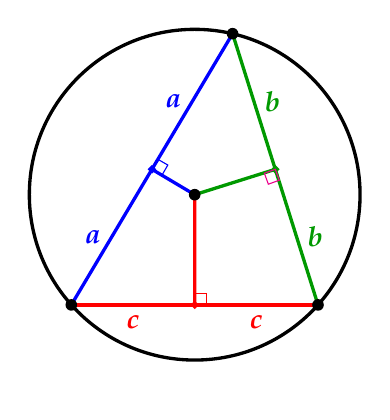
\begin{tikzpicture}[scale=.7,baseline=-25mm]
% Circle goes from (a) to (b)
\coordinate (a) at (0,0);
\coordinate (b) at (6,0);
% Line containing lower points is (c) -- (d)
\coordinate (c) at (0,-2);
\coordinate (d) at (6,-2);
% Line containing upper points is (e) -- (f)
\coordinate (e) at (0,2);
\coordinate (f) at (4,3);
% Name the two chords
\path [name path=chord1] (c) -- (d);
\path [name path=chord2] (e) -- (f);
% Name the coordinate of the center of the circle
\coordinate (center) at ($ (a)!.5!(b) $);
% Draw a circle whose center is half-way between (a) and (b) through (a)
\node [draw,very thick,circle through=(a),name path=circ] at (center) {};
% Get intersections of the upper and lower lines with the circle
\path [name intersections={of=circ and chord1,by={i1,i2}}];
\path [name intersections={of=circ and chord2,by={i3,i4}}];
% Draw triangle
\draw [very thick,blue] (i1) -- node[left] {$\bm{a}$} ($(i1)!.5!(i3)$) --
  node[left] {$\bm{a}$} (i3);
\draw[very thick,green!60!black] (i3) -- node[right] {$\bm{b}$} ($(i3)!.5!(i2)$) --
  node[right] {$\bm{b}$} (i2);
\draw[very thick,red] (i2) -- node[below] {$\bm{c}$} ($(i2)!.5!(i1)$) -- 
  node[below] {$\bm{c}$} (i1);
% Draw three perpendicular bisectors
\draw [very thick,red,fill] (center) -- ($(i1)!(center)!(i2)$)
  circle[radius=1pt];
\draw [very thick,blue,fill] (center) -- ($(i1)!(center)!(i3)$)
  circle[radius=1pt];
\draw [very thick,green!60!black,fill] (center) -- ($(i2)!(center)!(i3)$)
  circle[radius=1pt];
% Draw squares to denote right angles
\draw[red] ($ (i1) !.5! (i2) $) rectangle +(6pt,6pt);
\draw[blue,rotate=-30] ($ (i1) !.5! (i3) $) rectangle +(6pt,6pt);
\draw[magenta,rotate=-160] ($ (i3) !.5! (i2) $)
  rectangle +(6pt,6pt);
% Draw dots at all intersections
\fill (i1) circle (3pt);
\fill (i2) circle (3pt);
\fill (i3) circle (3pt);
\fill (center) circle (3pt);
\end{tikzpicture}

\smallskip\sffamily
\centering
Intersection of the perpendicular bisectors.
\end{minipage}

%%%%%%%%%%%%%%%%%%%%%%%%%%%%%%%%%%%%%%%%%%%%%%%%%%%%%%%%%%%%%%%%

\bigskip
\bigskip
\bigskip

\begin{center}
\Large\sffamily\bfseries Circles
\end{center}

%
% Inscribed angle one half of central angle
%
\begin{minipage}[t]{.45\textwidth}
\hspace{3em}
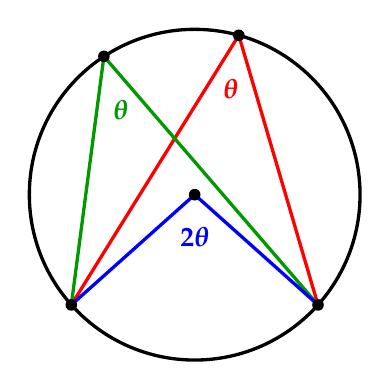
\begin{tikzpicture}[scale=.7]
% Circle goes from (a) to (b)
\coordinate (a) at (0,0);
\coordinate (b) at (6,0);
\coordinate (center) at (3,0);
% Line containing lower points is (c) -- (d)
\coordinate (c) at (0,-2);
\coordinate (d) at (6,-2);
% Line containing upper points is (e) -- (f);
\coordinate (e) at (0,2.3);
\coordinate (f) at (4.5,3);
% Name the upper and lower lines
\path [name path=chord1] (c) -- (d);
\path [name path=chord2] (e) -- (f);
% Draw a circle whose center is half-way between (a) and (b) through (a)
\node [draw,very thick,circle through=(a),name path=circ] at (center) {};
% Get intersections of the upper and lower lines with the circle
\path [name intersections={of=circ and chord1,by={i1,i2}}];
\path [name intersections={of=circ and chord2,by={i3,i4}}];
% Draw the lower chord
%\draw[very thick] (i1) -- (i2);
% Draw the two subtended angles and the center angle
\draw[very thick,red] (i1) -- (i3)
  node[below,xshift=-3pt,yshift=-12pt] {$\bm{\theta}$} -- (i2);
\draw[very thick,green!60!black] (i1) -- (i4)
  node[below,xshift=6pt,yshift=-12pt] {$\bm{\theta}$} -- (i2);
\draw[very thick,blue] (i1) -- (center)
  node[below,yshift=-8pt] {$\bm{2\theta}$} -- (i2);
% Dots at intersections
\fill (i1) circle (3pt);
\fill (i2) circle (3pt);
\fill (i3) circle (3pt);
\fill (i4) circle (3pt);
\fill (center) circle (3pt);
\end{tikzpicture}

\smallskip\sffamily
\centering
Central angle and inscribed angle.
\end{minipage}
%
\hspace{.1\textwidth}
% Angles of tangent and angle subtending a chord are equal
%
\begin{minipage}[t]{.45\textwidth}
\hspace{3em}
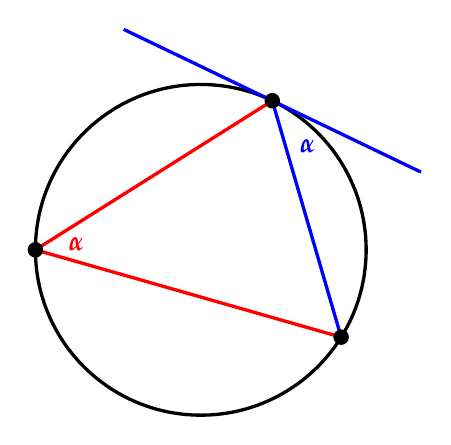
\begin{tikzpicture}[scale=.7,baseline=-60pt]
% Circle goes from (a) to (b)
\coordinate (a) at (0,0);
\coordinate (b) at (6,0);
% Line containing lower point (d)
\coordinate (d) at (7,-2);
% Point outside circle is (e)
\coordinate (e) at (1.6,4);
% Name the lower chord
\path [name path=chord] (a) -- (d);
% Draw a circle whose center is half-way between (a) and (b) through (a)
\node [draw,very thick,circle through=(a),name path=circ] (circle) at ($ (a)!.5!(b) $) {};
% Get intersection of the lower line with the circle
\path [name intersections={of=circ and chord,by={i1,i2}}];
% Draw the tangent line
\coordinate (tan) at (tangent cs:node=circle, point={(e)}, solution=2);
\draw[very thick,blue] (e) -- ($ (e)!2!(tan) $);
% Draw the triangle
\draw [very thick,blue] (tan) node[below right,xshift=6pt,yshift=-10pt] {$\bm{\alpha}$} -- (i2);
\draw [very thick,red] (tan) -- (a) node[right,xshift=8pt,yshift=2pt] {$\bm{\alpha}$} -- (i2);
% Dots at intersections
\fill (a) circle (4pt);
\fill (i2) circle (4pt);
\fill (tan) circle(4pt);
\end{tikzpicture}

\smallskip\sffamily
The angle subtending a chord and the angle between the chord and the tangent.
\end{minipage}

\bigskip
\bigskip

% Intersecting secants
%
\begin{minipage}[t]{.45\textwidth}
\hspace{4em}
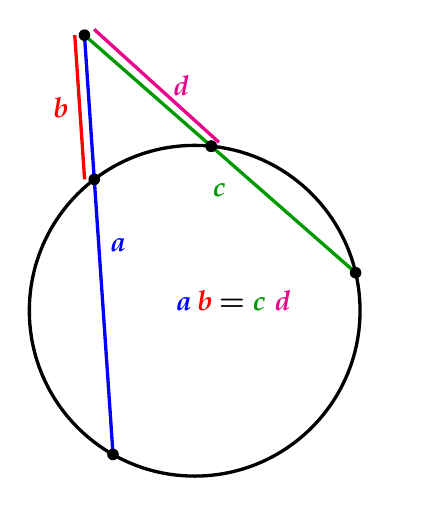
\begin{tikzpicture}[scale=.7]
% Circle goes from (a) to (b)
\coordinate (a) at (0,0);
\coordinate (b) at (6,0);
% Line containing lower points is (c) -- (d)
\coordinate (c) at (1,-3);
\coordinate (d) at (7,1.5);
% Point outside circle is (e)
\coordinate (e) at (1,5);
% Name the lower chord
\path [name path=chord] (c) -- (d);
% Draw a circle whose center is half-way between (a) and (b) through (a)
\node [draw,very thick,circle through=(a),name path=circ] at ($ (a)!.5!(b) $) {};
% Get intersection of the lower line with the circle
\path [name intersections={of=circ and chord,by={i1,i2}}];
% Draw the full secants
\draw [name path=secant1,very thick,green!60!black] (i1) -- node[left,xshift=6pt,yshift=-13pt] {$\bm{c}$} (e);
\draw [name path=secant2,very thick,blue] (i2) -- node[right] {$\bm{a}$} (e);
% Get intersections of the secants with the circle
\path [name intersections={of=circ and secant1,by={s11,s12}}];
\path [name intersections={of=circ and secant2,by={s21,s22}}];
% Draw offset lines from outside point with the intersections of the secants
\draw[very thick,red]
  let \p1 = (s21), \p2 = (e) in
    (\x2-5pt,\y2) -- node[left] {$\bm{b}$} (\x1-5pt,\y1);
\draw[very thick,magenta]
  let \p1 = (s12), \p2 = (e) in
    (\x2+5pt,\y2+3pt) -- node[right,xshift=2pt] {$\bm{d}$} (\x1+4pt,\y1+2pt);
% Dots at intersections
\fill (s11) circle (3pt);
\fill (s12) circle (3pt);
\fill (s21) circle (3pt);
\fill (s22) circle (3pt);
\fill (s12) circle (3pt);
\fill (e) circle (3pt);
% Display formula in color
\begin{scope}[xshift=2.8cm]
\node[anchor=base,blue] at (0,0) {$\bm{a}$};
\node[anchor=base,red] at (11pt,0) {$\bm{b}$};
\node[anchor=base] at (25pt,0) {$\bm{=}$};
\node[anchor=base,green!60!black] at (39pt,0) {$\bm{c}$};
\node[anchor=base,magenta] at (51pt,0) {$\bm{d}$};
\end{scope}
\end{tikzpicture}

\smallskip\sffamily
\centering
Intersecting secants.
\end{minipage}
\hspace{.1\textwidth}
%
% Intersecting tangent and secant
%
\begin{minipage}[t]{.45\textwidth}
\hspace{4em}
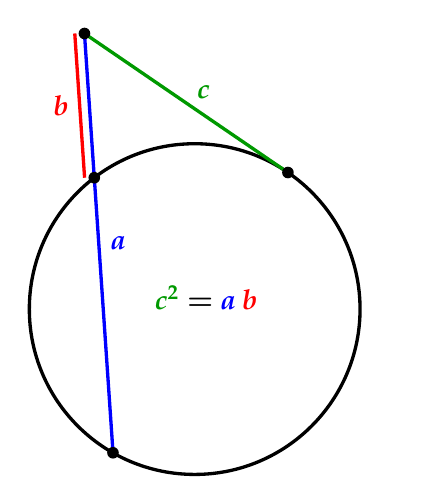
\begin{tikzpicture}[scale=.7]
% Circle goes from (a) to (b)
\coordinate (a) at (0,0);
\coordinate (b) at (6,0);
% Line containing lower points is (c) -- (d)
\coordinate (c) at (1,-3);
\coordinate (d) at (7,1.5);
% Point outside circle is (e)
\coordinate (e) at (1,5);
% Name the lower chord
\path [name path=chord] (c) -- (d);
% Draw a circle whose center is half-way between (a) and (b) through (a)
\node [draw,very thick,circle through=(a),name path=circ] (circle) at ($ (a)!.5!(b) $) {};
% Get intersection of the lower line with the circle
\path [name intersections={of=circ and chord,by={i1,i2}}];
% Draw the full secant
\draw [name path=secant2,very thick,blue] (i2) -- node[right] {$\bm{a}$} (e);
% Get intersection of the secant with the circle
\path [name intersections={of=circ and secant2,by={s21,s22}}];
% Draw offset line from outside point with the intersection of the secant
\draw[very thick,red]
  let \p1 = (s21), \p2 = (e) in
    (\x2-5pt,\y2) -- node[left] {$\bm{b}$} (\x1-5pt,\y1);
% Draw the tangent line
\coordinate (tan) at (tangent cs:node=circle, point={(e)}, solution=2);
\draw[very thick,green!60!black] (e) -- node[right,yshift=4pt] {$\bm{c}$} (tan);
% Dots at intersections
\fill (s21) circle (3pt);
\fill (s22) circle (3pt);
\fill (e) circle (3pt);
\fill (tan) circle(3pt);
% Display formula in color
\begin{scope}[xshift=2.5cm]
\node[anchor=base,green!60!black] at (0,0) {$\bm{c^2}$};
\node[anchor=base] at (.6,0) {$\bm{=}$};
\node[anchor=base,blue] at (1.1,0) {$\bm{a}$};
\node[anchor=base,red] at (1.5,0) {$\bm{b}$};
\end{scope}
\end{tikzpicture}

\smallskip\sffamily
\centering
Intersecting secant and tangent.
\end{minipage}

\bigskip
\bigskip

% Intersecting chords
%
\begin{minipage}[t]{.45\textwidth}
\hspace{4em}
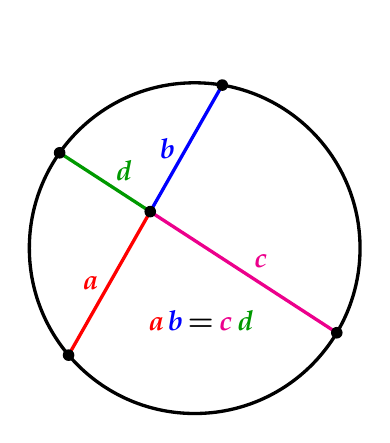
\begin{tikzpicture}[scale=.7]
% Circle goes from (a) to (b)
\coordinate (a) at (0,0);
\coordinate (b) at (6,0);
% Line containing lower points is (c) -- (d)
\coordinate (c) at (0,-2);
\coordinate (d) at (6,-1.5);
% Line containing upper points is (e) -- (f)
\coordinate (e) at (0,1.5);
\coordinate (f) at (6,4);
% Name the upper and lower lines
\path [name path=chord1] (c) -- (d);
\path [name path=chord2] (e) -- (f);
% Draw a circle whose center is half-way between (a) and (b) through (a)
\node [draw,very thick,circle through=(a),name path=circ] at ($ (a)!.5!(b) $) {};
% Get intersections of the upper and lower lines with the circle
\path [name intersections={of=circ and chord1,by={i1,i2}}];
\path [name intersections={of=circ and chord2,by={i3,i4}}];
% Name the two chords
\path [name path=x1] (i1) -- (i3);
\path [name path=x2] (i2) -- (i4);
% Get their intersection
\path [name intersections={of=x1 and x2,by={p}}];
% Draw four lines from intersection to circle
\draw[very thick,red] (i1) -- node[left] {$\bm{a}$} (p);
\draw[very thick,blue] (p) --  node[left] {$\bm{b}$} (i3);
\draw[very thick,magenta] (i2) -- node[right,yshift=4pt] {$\bm{c}$} (p);
\draw[very thick,green!60!black] (p) -- node[right,yshift=4pt] {$\bm{d}$} (i4);
% Dots at intersections
\fill (p) circle (3pt);
\fill (i1) circle (3pt);
\fill (i2) circle (3pt);
\fill (i3) circle (3pt);
\fill (i4) circle (3pt);
% Display formula in color
\begin{scope}[xshift=2.3cm,yshift=-1.5cm]
\node[anchor=base,red] at (0,0) {$\bm{a}$};
\node[anchor=base,blue] at (10pt,0) {$\bm{b}$};
\node[anchor=base] at (23pt,0) {$\bm{=}$};
\node[anchor=base,magenta] at (36pt,0) {$\bm{c}$};
\node[anchor=base,green!60!black] at (46pt,0) {$\bm{d}$};
\end{scope}
\end{tikzpicture}

\smallskip\sffamily
\centering Intersecting chords
\end{minipage}
\hspace{.1\textwidth}
%
% Intersecting tangents
%
\begin{minipage}[t]{.45\textwidth}
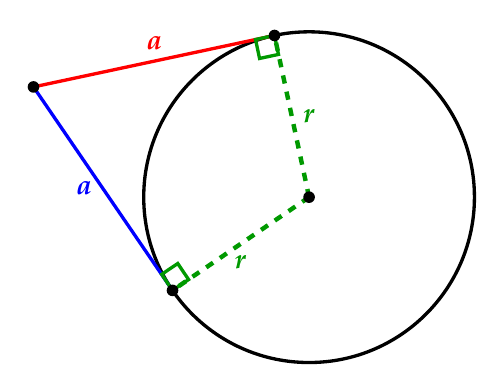
\begin{tikzpicture}[scale=.7]
% Circle goes from (a) to (b)
\coordinate (a) at (0,0);
\coordinate (b) at (6,0);
\coordinate (center) at (3,0);
% Point outside circle is (e)
\coordinate (e) at (-2,2);
\node [draw,very thick,circle through=(a),name path=circ] (circle) at (center) {};
% Draw the tangent line
\coordinate (tan1) at (tangent cs:node=circle, point={(e)}, solution=1);
\coordinate (tan2) at (tangent cs:node=circle, point={(e)}, solution=2);
\draw[very thick,blue] (e) -- node[left] {$\bm{a}$} (tan1);
\draw[very thick,red] (e) -- node[above] {$\bm{a}$} (tan2);
% Draw radii
\draw[ultra thick,dashed,green!60!black] (center) -- node[below] {$\bm{r}$} (tan1);
\draw[ultra thick,dashed,green!60!black] (center) -- node[right] {$\bm{r}$} (tan2);
% Draw right angles
\draw[very thick,green!60!black,rotate=34] (tan1) rectangle +(10pt,10pt);
\draw[very thick,green!60!black,rotate=-168] (tan2) rectangle +(10pt,10pt);
% Dots at intersections
\fill (e) circle (3pt);
\fill (center) circle (3pt);
\fill (tan1) circle(3pt);
\fill (tan2) circle(3pt);
\end{tikzpicture}

\smallskip\sffamily
\centering
Intersecting tangents.
\end{minipage}

%%%%%%%%%%%%%%%%%%%%%%%%%%%%%%%%%%%%%%%%%%%%%%%%%%%%%%%%%%

\bigskip
\bigskip
\bigskip


\begin{center}
\Large\sffamily\bfseries Quadrilaterals
\end{center}

%
% Sums of opposite sides of circumscribed quadrilateral are equal
%
\begin{minipage}[t]{.45\textwidth}
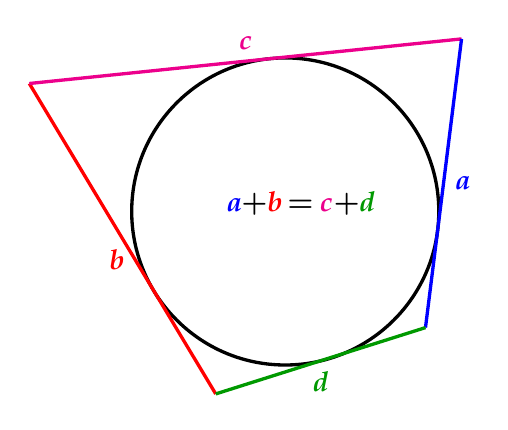
\begin{tikzpicture}[scale=.65]
% Circle goes from (a) to (b)
\coordinate (x) at (0,3);
\coordinate (y) at (6,3);
\coordinate (a) at (-2,5.5);
% Draw a circle whose center is half-way between (a) and (b) through (a)
\node [draw,very thick,circle through=(x),name path=circ] (circle) at ($ (x)!.5!(y) $) {};
% Draw tangent lines
\coordinate (tan1) at (tangent cs:node=circle, point={(a)}, solution=1);
\draw[very thick,red] (a) -- node[below,xshift=-2pt] {$\bm{b}$}
  ($(a)!1.5!(tan1)$) coordinate (b);
\coordinate (tan2) at (tangent cs:node=circle, point={(a)}, solution=2);
\draw[very thick,magenta] (a) -- node[above] {$\bm{c}$}
  ($(a)!1.8!(tan2)$) coordinate (c);
\coordinate (tan3) at (tangent cs:node=circle, point={(c)}, solution=2);
\draw[very thick,blue] (c) -- node[right] {$\bm{a}$}
  ($(c)!1.51!(tan3)$)  coordinate (d);
\draw[very thick,green!60!black] (b) -- node[below] {$\bm{d}$} (d);
% Display formula in color
\begin{scope}[xshift=2cm,yshift=3cm]
\node[anchor=base,blue] at (0,0) {$\bm{a}$};
\node[anchor=base] at (.4,0) {$\bm{+}$};
\node[anchor=base,red] at (.8,0) {$\bm{b}$};
\node[anchor=base] at (1.3,0) {$\bm{=}$};
\node[anchor=base,magenta] at (1.8,0) {$\bm{c}$};
\node[anchor=base] at (2.2,0) {$\bm{+}$};
\node[anchor=base,green!60!black] at (2.6,0) {$\bm{d}$};
\end{scope}
\end{tikzpicture}

\smallskip\sffamily
Opposite sides of a circumscribed quadrilateral.
\end{minipage}
\hspace{.1\textwidth}
%
% Opposite angles in an inscribed quadrilateral add up to 180
%
\begin{minipage}[t]{.45\textwidth}
\hspace{4em}
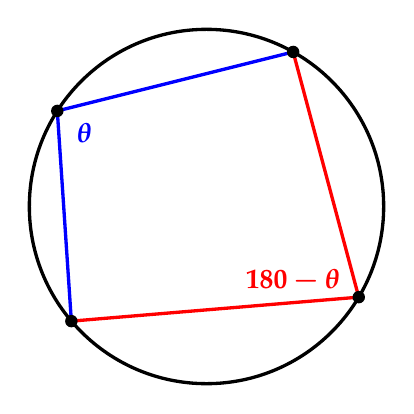
\begin{tikzpicture}[scale=.75]
% Circle goes from (a) to (b)
\coordinate (a) at (0,0);
\coordinate (b) at (6,0);
% Line containing lower points is (c) -- (d)
\coordinate (c) at (0,-2);
\coordinate (d) at (6,-1.5);
% Line containing upper points is (e) -- (f)
\coordinate (e) at (0,1.5);
\coordinate (f) at (6,3);
% Name the upper and lower lines
\path [name path=chord1] (c) -- (d);
\path [name path=chord2] (e) -- (f);
% Draw a circle whose center is half-way between (a) and (b) through (a)
\node [draw,very thick,circle through=(a),name path=circ] at ($ (a)!.5!(b) $) {};
% Get intersections of the upper and lower lines with the circle
\path [name intersections={of=circ and chord1,by={i1,i2}}];
\path [name intersections={of=circ and chord2,by={i3,i4}}];
% Draw the two subtended angles
\draw[very thick,red] (i1) -- (i2)
  node[left,xshift=-3pt,yshift=6pt] {$\bm{180-\theta}$} -- (i3);
\draw[very thick,blue] (i1) -- (i4)
  node[right,xshift=3pt,yshift=-8pt] {$\bm{\theta}$} -- (i3);
% Dots at intersections
\fill (i1) circle (3pt);
\fill (i2) circle (3pt);
\fill (i3) circle (3pt);
\fill (i4) circle (3pt);
\end{tikzpicture}

\smallskip\sffamily
Opposite angles of an inscribed quadrilateral.
\end{minipage}

\bigskip
\bigskip

% Diagonals of parallelogram bisect each other
%
\begin{minipage}[t]{.45\textwidth}
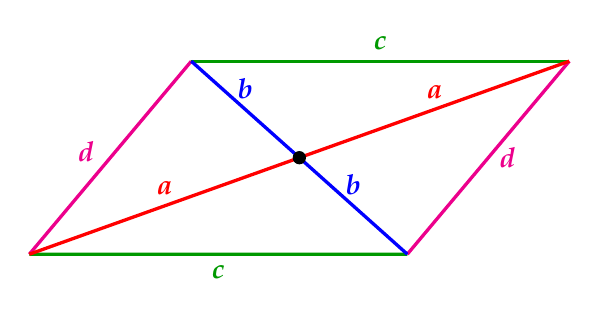
\begin{tikzpicture}[scale=.8]
% Bottom side of parallelogram
\coordinate (a) at (0,0);
\coordinate (b) at (6,0);
% Draw parallelogram at angle 50
\draw[very thick,magenta] (a) -- node[left,xshift=-2pt,yshift=2pt] {$\bm{d}$} +(50:4) coordinate (c);
\draw[very thick,green!60!black] (c) -- node[above] {$\bm{c}$} +(6,0) coordinate (d);
\draw[very thick,magenta] (d) -- node[right] {$\bm{d}$} +(230:4) coordinate (b);
\draw[very thick,green!60!black] (b) -- node[below] {$\bm{c}$} (a);
% Name the two diagonals
\path [name path=d1] (a) -- (d);
\path [name path=d2] (b) -- (c);
% Get their intersection
\path [name intersections={of=d1 and d2,by={intersection}}];
% Draw diagonals
\draw[very thick,red] (a) -- node[above] {$\bm{a}$} (intersection);
\draw[very thick,red] (intersection) -- node[above] {$\bm{a}$} (d);
\draw[very thick,blue] (b) -- node[above] {$\bm{b}$} (intersection);
\draw[very thick,blue] (intersection) -- node[above] {$\bm{b}$} (c);
% Dot at their intersection
\fill (intersection) circle (3pt);
\end{tikzpicture}

\smallskip\sffamily
\centering
Diagonals of a parallelogram.
\end{minipage}
%
\hspace{.1\textwidth}
%
% Diagonals of rhombus bisect each other and are perpendicular
%
\begin{minipage}[t]{.45\textwidth}
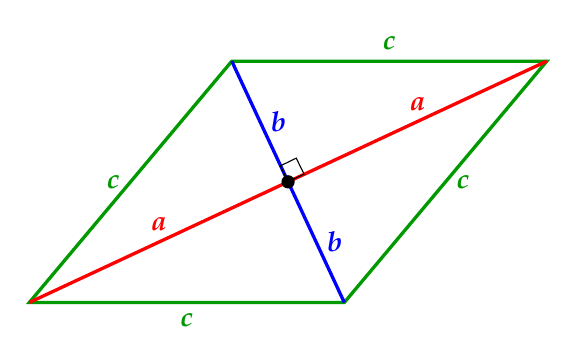
\begin{tikzpicture}[scale=.8]
% Bottom side of rhombus
\coordinate (a) at (0,0);
\coordinate (b) at (5,0);
% Draw rhombus at angle 50
\draw[very thick,green!60!black] (a) -- node[left] {$\bm{c}$} ++(50:5) coordinate (c) -- node[above] {$\bm{c}$} ++(5,0) coordinate (d) -- node[right] {$\bm{c}$} (b) -- node[below] {$\bm{c}$} cycle;
% Name the two diagonals
\path [name path=d1] (a) -- (d);
\path [name path=d2] (b) -- (c);
% Get their intersection
\path [name intersections={of=d1 and d2,by={intersection}}];
% Draw diagonals
\draw[very thick,red] (a) -- node[above] {$\bm{a}$} (intersection);
\draw[very thick,red] (intersection) -- node[above] {$\bm{a}$} (d);
\draw[very thick,blue] (b) -- node[right] {$\bm{b}$} (intersection);
\draw[very thick,blue] (intersection) -- node[right] {$\bm{b}$} (c);
% Draw square to denote right angle
\draw[rotate=26] (intersection) rectangle +(8pt,8pt);
% Dot at their intersection
\fill (intersection) circle (3pt);
\end{tikzpicture}

\smallskip\sffamily
\centering
Diagonals of a rhombus.
\end{minipage}

\bigskip
\bigskip

%
% Median of a trapezoid is average of sides
%
\begin{minipage}[t]{.45\textwidth}
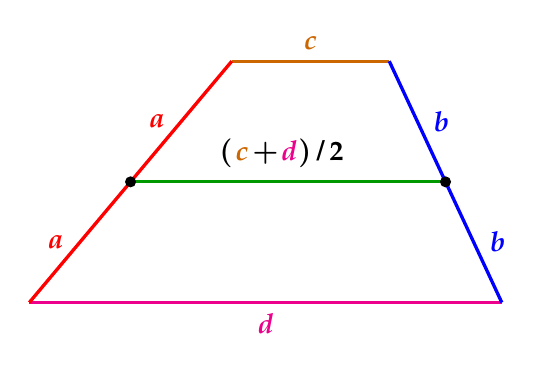
\begin{tikzpicture}
% Bottom of trapeze
\coordinate (a) at (0,0);
\coordinate (b) at (6,0);
% Draw the bases of the trapeze
\draw[very thick,magenta] (a) -- node[below] {$\bm{d}$} (b);
\path (a) -- ++(50:4) coordinate (c) -- ++(2,0) coordinate (d);
\draw[very thick,orange!80!black] (c) -- node[above] {$\bm{c}$} (d);
% Draw the sides of the trapeze in two parts
\coordinate (mid1) at ($(a)!.5!(c)$);
\coordinate (mid2) at ($(b)!.5!(d)$);
\draw[very thick,red] (a) -- node[left,xshift=-2pt] {$\bm{a}$} (mid1);
\draw[very thick,red] (mid1) -- node[left,xshift=-2pt] {$\bm{a}$} (c);
\draw[very thick,blue] (b) -- node[right,xshift=2pt] {$\bm{b}$} (mid2);
\draw[very thick,blue] (mid2) -- node[right,xshift=2pt] {$\bm{b}$} (d);
% Draw the median
\draw[very thick,green!60!black] (mid1) -- (mid2);
% Display formula in color
\begin{scope}[xshift=25mm,yshift=18mm]
\node[anchor=base] at (0,0) {$\bm{(}$};
\node[anchor=base,orange!80!black] at (.2,0) {$\bm{c}$};
\node[anchor=base] at (.5,0) {$\bm{+}$};
\node[anchor=base,magenta] at (.8,0) {$\bm{d}$};
\node[anchor=base] at (1.0,0) {$\bm{)}$};
\node[anchor=base] at (1.2,0) {$\bm{/}$};
\node[anchor=base] at (1.4,0) {$\bm{2}$};
\end{scope}

% Dots at the midpoints
\fill (mid1) circle (2pt);
\fill (mid2) circle (2pt);
\end{tikzpicture}

\smallskip\sffamily
\centering
Median of a trapezoid.
\end{minipage}
%
\hspace{.1\textwidth}
%
% Diagonals of a kite
%
\begin{minipage}[t]{.45\textwidth}
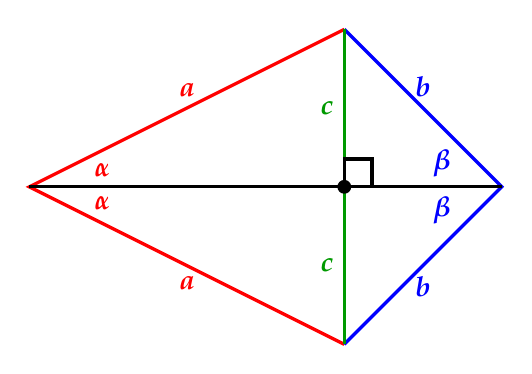
\begin{tikzpicture}[scale=1]
% Draw the kite
\coordinate (a) at (0,0);
\coordinate (b) at (4,2);
\coordinate (c) at (6,0);
\coordinate (d) at (4,-2);
\coordinate (intersection) at (4,0);
\draw[red,very thick] (d) -- node[below] {$\bm{a}$} (a) -- node[above] {$\bm{a}$} (b);
\draw[blue,very thick] (b) -- node[above] {$\bm{b}$} (c) -- node[below] {$\bm{b}$} (d);
% Label nodes
\node[red,above right,xshift=20pt] at (a) {$\bm{\alpha}$};
\node[red,below right,xshift=20pt] at (a) {$\bm{\alpha}$};
\node[blue,above left,xshift=-15pt] at (c) {$\bm{\beta}$};
\node[blue,below left,xshift=-15pt] at (c) {$\bm{\beta}$};
% Draw diagonals
\draw[very thick] (a) -- (c);
\draw[green!60!black,very thick] (b) -- node[left] {$\bm{c}$}(intersection) -- node[left] {$\bm{c}$} (d);
\fill (intersection) circle (2.5pt);
% Draw square to denote right angle
\draw[very thick] (intersection) rectangle +(10pt,10pt);
\end{tikzpicture}

\smallskip\sffamily
\centering
Diagonals of a kite.
\end{minipage}
\end{document}
